\section{Validating the code}

\subsection{Calculation for non-interacting particles}

For non-interacting particles in a Quantum Dot, no Jastrow factor and $\alpha=1$ provides the exact wave function. This serves as a powerful guide, since results can be benchmarked against exact solutions. In the non-interacting case, the minimization should always yield $\alpha=1$.

Let $R$ denote the highest filled \textit{shell}, i.e. the maximum value of $n_x + n_y$, $N_j$ be the number of particles in a given shell ($1\le j\le R$), $\chi$ be the spin levels and $\epsilon_i = i\omega$, where $i=n_x + n_y$, is the single particle energy at shell level $i$. Then the non-interacting energy of a closed shell Quantum Dot is

\begin{align}
 E_0 &= \sum_\chi\sum_{i=1}^R\sum_{j=1}^{N_i} \epsilon_i \\
     &= 2\sum_{i=1}^R N_i i \omega 
\end{align}

Realizing that (not counting spin) $N_i = i$ for a Quantum Dot, we get

\begin{align}
 E_0 &= 2\omega\sum_{i=1}^R i^2 \\
     &= 2\omega \left(\frac{1}{6}R(R+1)(2R + 1)\right) \\
     &= \frac{R}{3}(R + 1)(2R + 1)\omega
\end{align}

which tabulated for the lowest lying shells yields

\begin{center}
 \begin{tabular}{cc|c}
 R & N  & $E_0/\omega$ \\
 \hline
 1 & 2  & 2  \\
 2 & 6  & 10 \\
 3 & 12 & 28 \\
 4 & 20 & 60 \\
 5 & 30 & 110\\
 6 & 42 & 182\\
 \end{tabular}
\end{center}

The first step to validating the code would be to reproduce these exact results. The minimization method should seek an $\alpha$ close to one, where the variational derivative should be zero. In Table \ref{tab:res_valid_qdots}, validation runs for the three lowest shells are run. Figure \ref{fig:ASGD_nonint} shows the ASGD method finding the minima.


\begin{table}
\begin{center}
\begin{tabular}{cc|cccc}
    N     & $\omega$ & $\mathrm{E_{VMC}}$ & $\mathrm{E_{DMC}}$ & $\alpha$ & $E_0$ \\
\hline
    2     &   0.5    &   1.0    &   1.0    &   1.0    & 1 \\
          &   1.0    &   2.0    &   2.0    &   1.0    & 2 \\
    6     &   0.5    &   5.0    &   5.0    &   1.0    & 5 \\
          &   1.0    &   10.0   &   10.0   &   1.0    & 10 \\
    12    &   0.5    &   14.0   &   14.0   &   1.0    & 14 \\
          &   1.0    &   28.0   &   28.0   &   1.0    & 28 \\
\end{tabular}
\caption{Validation results for Quantum Dots generated using 2000 to 3000 ASGD cycles starting from $\alpha=0.5$. The sampled variance from DMC and VMC is of order $10^{-16}$ (non-zero due to small deviations in $\alpha$ from unity). The last column lists the exact energies. As required we have an exact match (to machine precision). Hard coding $\alpha=1.0$ will yield zero variance.}
\label{tab:res_valid_qdots}
\end{center}
\end{table}


\begin{figure}
 \begin{center}
  \subfigure{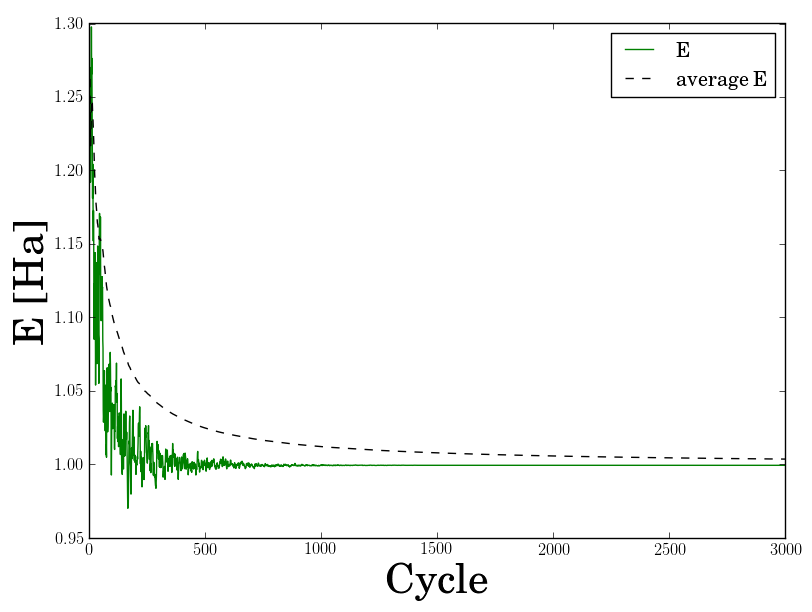
\includegraphics[scale=0.37]{../Graphics/ASGD_nonint_E.png}}
  \subfigure{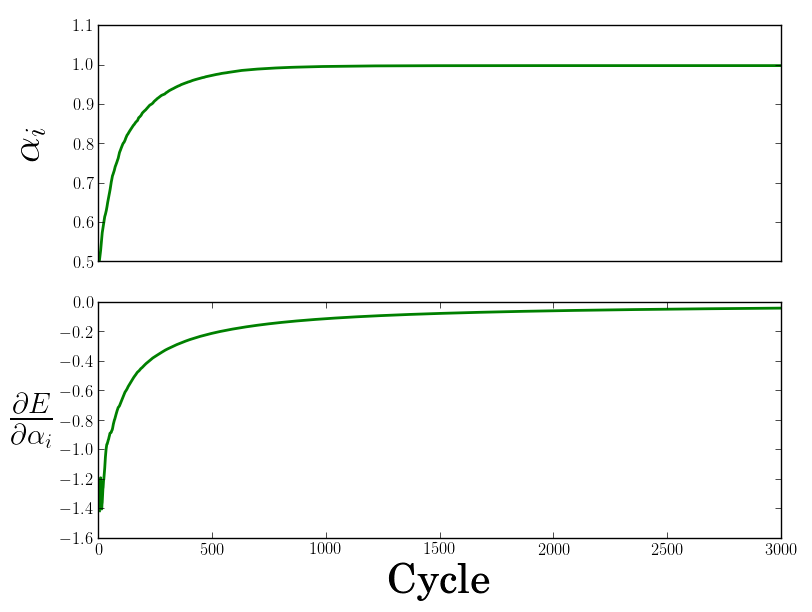
\includegraphics[scale=0.37]{../Graphics/ASGD_nonint.png}} 
  \caption{ASGD results for a non-interaction two-particle Quantum Dot with $\omega=0.5$. The exact energy of $E_0=1$ is reached after approximatly 1000 cycles, where $\alpha$ has converged close to unity. Due to enormous fluctuations, the variational derivative is plotted as an accumulated average, and is in practice dead zero after 1000 cycles. The variational principle described in Section \ref{sec:selectingOptVarPar} is governing the trend of the energy convergence, however, alot of statistical noise is present in the first 1000 cycles due to high variance and few samples.}
  \label{fig:ASGD_nonint}
 \end{center}
\end{figure}

Similar validation can be done for atoms, and is listed in Table \ref{tab:res_valid_atoms}. The non-interaction energy is given by the following expression

\begin{equation}
 E_0 = -\frac{N^2}{2}\sum_{i=1}^N \frac{1}{n_i^2}
\end{equation}


\begin{table}
\begin{center}
\begin{tabular}{c|cccc}
    N     & $\mathrm{E_{VMC}}$ & $\mathrm{E_{DMC}}$ & $\alpha$ & $E_0$\\
\hline
    2     &   -4.0   &   -4.0   &   1.0  & -4  \\
    4     &  -20.0   &  -20.0   &   1.0  & -20 \\
    10    &  -200.0  &  -200.0  &   1.0  & -200\\
\end{tabular}
\caption{Validation results for Atoms generated in a similar way to the Quantum Dots results in Table \ref{tab:res_valid_qdots}.}
\label{tab:res_valid_atoms}
\end{center}
\end{table}

The DMC method in case of an exact wave function should do nothing. The trial energy should equal the ground state energy through all time steps and zero fluctuations in the number of walkers should occur. This trend is shown for Neon in Fig. \ref{fig:DMC_neon_nonint}.

\begin{figure}
 \begin{center}
  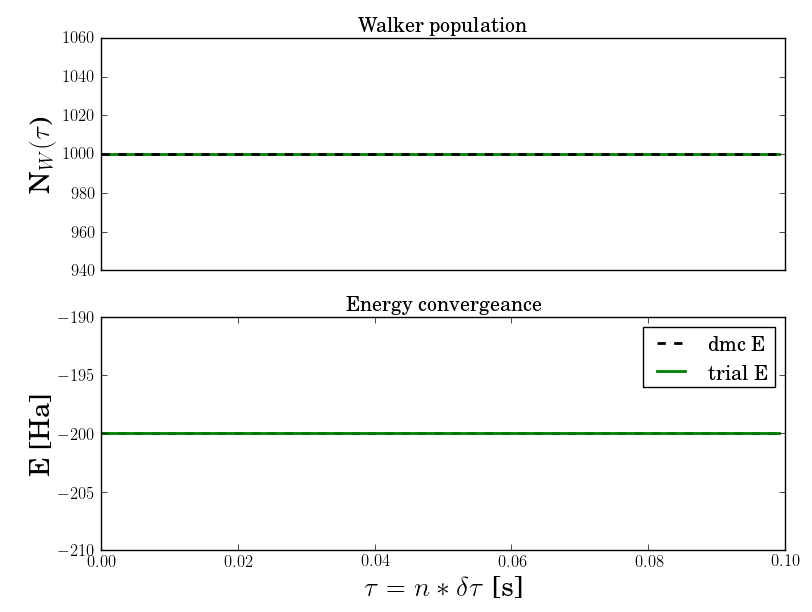
\includegraphics[scale=0.5]{../Graphics/DMC_neon_valid.png}
  \caption{DMC convergence for the Neon result listed in Table \ref{tab:res_valid_atoms}. The trial energy is fixed at the exact ground state energy as expected. The number of walkers are constant, implying a approximatly zero variance.}
  \label{fig:DMC_neon_nonint}
 \end{center}
\end{figure}

A final non-interacting case to run is the case of DMC without the exact wave function. As discussed in Chapter \ref{ch:QMC}, DMC should result in a better estimate of the ground state energy than VMC in case of a trial wave function different from the exact grouns state. A test-case is presented in Fig. \ref{fig:DMC_nonExactWF}.

\begin{figure}
 \begin{center}
  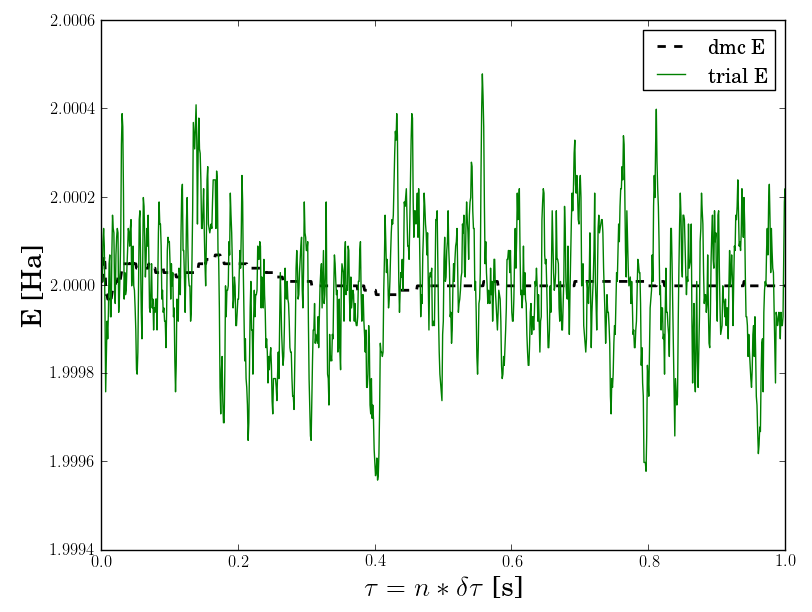
\includegraphics[scale=0.5]{../Graphics/DMC_notExactWF.png}
  \caption{DMC convergence for a non-interacting two-particle Quantum Dot with $\omega=1$. Calculations are done with $\alpha=0.75$, where the exact wave function is given for $\alpha=1$. Unlike the case with the exact wave function, the trial energy oscillates around the exact value. The final result (with blocking) reveals a DMC energy of $2.00000(2)$, where the original VMC energy was $2.0042(3)$. This illustrates the power of DMC over VMC in the interesting cases with an unknown exact wave function. The calculation were done with $10000$ walkers.}
  \label{fig:DMC_nonExactWF}
 \end{center}
\end{figure}